\documentclass[conference,compsoc]{IEEEtran}


% *** CITATION PACKAGES ***
%
\ifCLASSOPTIONcompsoc
  \usepackage[nocompress]{cite}
\else
  \usepackage{cite}
\fi

% *** GRAPHICS RELATED PACKAGES ***
%
\ifCLASSINFOpdf
\else
\fi

\hyphenation{op-tical net-works semi-conduc-tor}
\usepackage{graphicx}
\graphicspath{ {./img/} }


\begin{document}
\title{Convolutional Neural Network:\\ Leaves Classification
\\ \large Artificial Neural Networks and Deep Learning - a.y. 2021/2022}

\author{\IEEEauthorblockN{\textbf{Fabio Tresoldi}}
\IEEEauthorblockA{M.Sc. Computer Science and Engineering\\
Politecnico di Milano - Milan, Italy \\
E-mail: fabio1.tresoldi@mail.polimi.it \\
Student ID : 10607540 \\
Codalab Nickname: "fabioow" \\
Codalab Group: "artificial\_comrades"}
\and
\IEEEauthorblockN{\textbf{Mirko Usuelli}}
\IEEEauthorblockA{M.Sc. Computer Science and Engineering\\
Politecnico di Milano - Milan, Italy \\
E-mail: mirko.usuelli@mail.polimi.it \\
Student ID : 10570238 \\
Codalab Nickname: "mirko" \\
Codalab Group: "artificial\_comrades"}}

\maketitle

\begin{abstract}
In this report, we explore and compare the development process we had to design a Convolutional Neural Network able to classify 14 different plants species through their leaves images as input.
\end{abstract}
\IEEEpeerreviewmaketitle

\section{Introduction}
The given dataset is unbalanced with respect to the classes distribution, then we decided to apply a Stratified Sampling procedure in order to preserve the full dataset proportions both in training, validation and testing.

This structural characteristic suggests the usage of the Categorical Crossentropy as loss function, whereas as metrics we kept into account accuracy and F1-score, being the latter more meaningful for unbalanced categories, while the former is used for validation comparisons in this report.

\begin{figure}[h!]
\centering
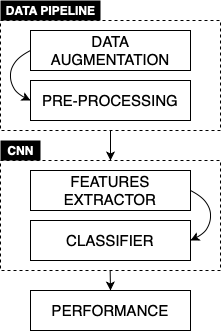
\includegraphics[width=1.9in]{img/development.png}
\caption{Development Process.}
\label{fig_sim}
\end{figure}

\section{Data Pipeline}
\subsection{Data Augmentation}
Due to the reduced dimension of the proposed dataset compared to the parameters complexity of the underlying architecture, Data Augmentation purpouse consists in solving this issue by generating at run time several new transformed images which allow a better generalized performance of the model. \\
Starting from Traditional Transformations (2.1.1), we tried to furtherly improved the quality of classification by introducing some Advanced Transformations (2.1.2).
\subsubsection{Traditional Transformations}
Rotating, Zooming, Flipping, Brightness, Shifting.
\subsubsection{Advanced Transformations}
CutMix, MixUp, CutOut.

However, these last Advance Transformations did not increased the overall performance in our specific case, but indeed, they made the training process slower and not as accurate as without them, therefore we decided to discard these techniques.

In terms of validation accuracy, within 20 epochs:

\begin{center}
\begin{tabular}{ c c }
\hline\hline
 No Augmentation & 99.86\% \\ 
\hline
 Traditional Transf. & \textbf{99.93\%}  \\  
 Advanced Transf. & 99.79\% \\
\hline\hline
\end{tabular}
\end{center}

\begin{figure}[h!]
\centering
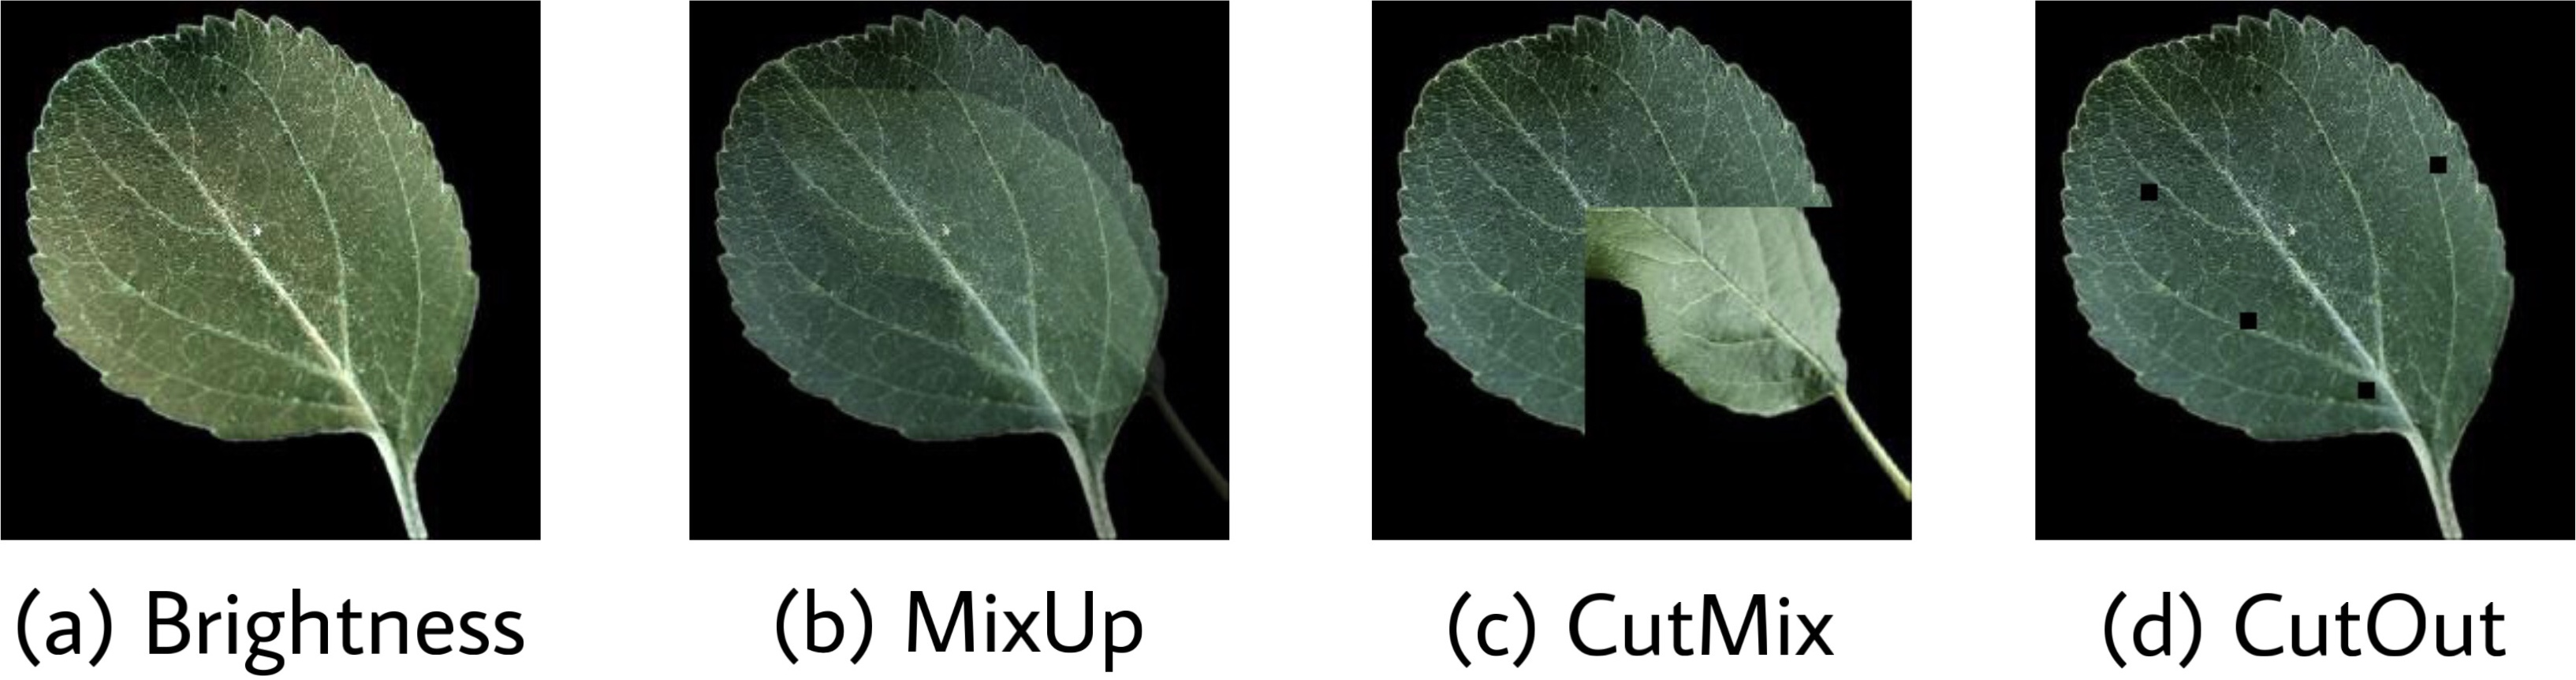
\includegraphics[width=3.1in]{img/leaves.jpg}
\caption{Some examples of Data Augmentation techniques.}
\label{fig_sim}
\end{figure}

\subsection{Pre-Processing}
Since for the Features Exctractor (section 3.1) we relied on State-of-Art architectures through Fine Tuning, the data pre-processing function adopted is the same suggested by the corresponding model contained in \texttt{tensorflow.keras.applications}.

\section{Convolutional Neural Network}
\subsection{Features Extractor}
We started comparing the most famous architectures showed during the course lectures through Transfer Learning and a simply GAP + Softmax layers as baseline classifier. Then we plotted both Categorical Crossentropy loss and Accuracy for the validation and training set (dashed line) within 10 epochs:

\begin{figure}[h!]
\centering
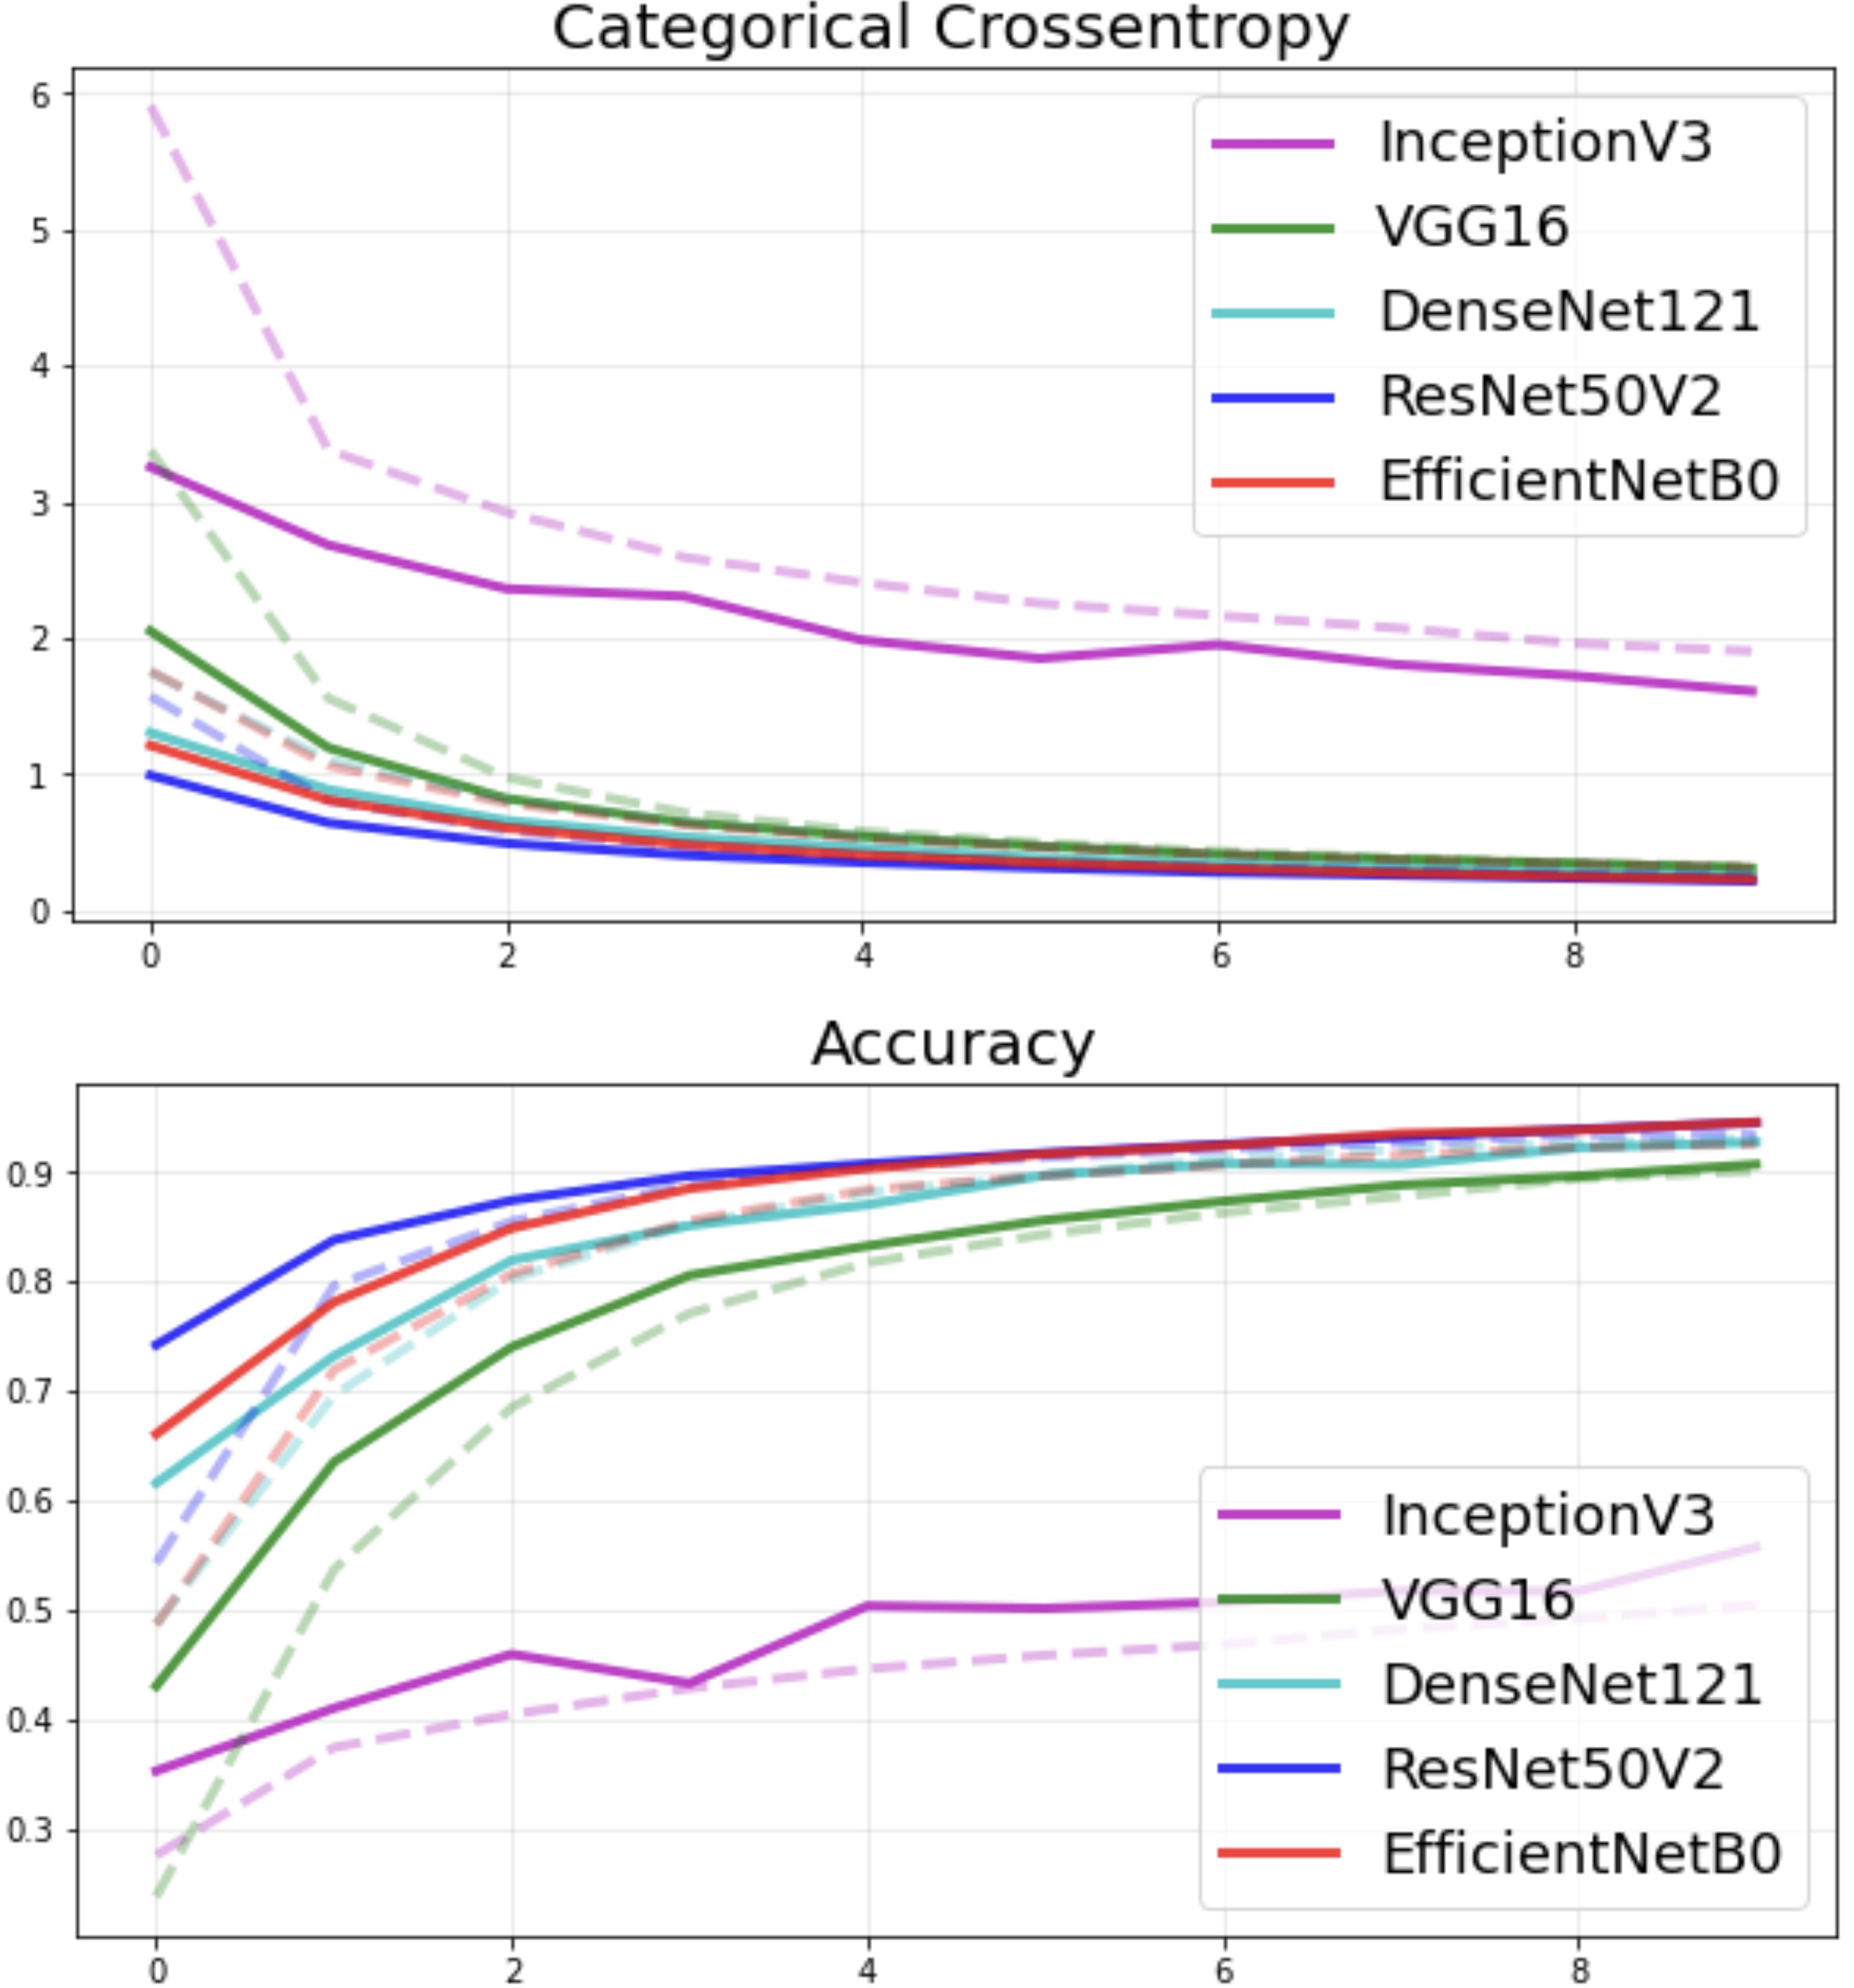
\includegraphics[width=3.1in]{img/comparison.jpg}
\caption{State-of-Art architectures comparison.}
\label{fig_sim}
\end{figure}

As shown in Figure 3, the best models were EfficientNet and ResNet. While the latter converges faster, the former is able to reach a higher peak of performance in both loss and metrics as epochs go further. Thus, we have chosen EfficientNet as Features Extractor.

\begin{center}
\begin{tabular}{ c c }
\hline\hline
 ResNet50V2 & 94.54\% \\ 
\hline
 EfficientNetB0 & \textbf{94.57\%}  \\  
 EfficientNetB1 & 94.40\%  \\
 EfficientNetB2 & 94.38\% \\
\hline\hline
\end{tabular}
\end{center}

\subsubsection{Ensemble}
Then we started introducing the concept of Ensemble in order to reduce the overall variance in prediction. By taking the input multiple times through different Features Extractors, we concatenated the GAP ouput for each model in purpose to feed the final classifier with different conclusions.

\begin{figure}[h!]
\centering
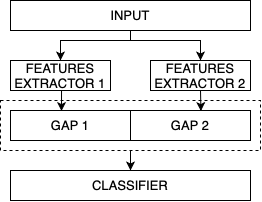
\includegraphics[width=2.5in]{img/ensemble.png}
\caption{CNN Ensemble.}
\label{fig_sim}
\end{figure}

However, this method performed worse than a single CNN, therefore we discarded this technique.

\begin{center}
\begin{tabular}{ c c }
\hline\hline
 EfficientNetB0 & \textbf{99.97\%}  \\  
 EfficientNetB0+B1 & 99.92\%  \\
 EfficientNetB0+B1+B2 & 99.88\% \\
\hline\hline
\end{tabular}
\end{center}

\subsection{Classifier}
Starting from a general classifier model, with the main layers shown during the course, we analyzed the performance of each of them through Transfer Learning:

\begin{figure}[h!]
\centering
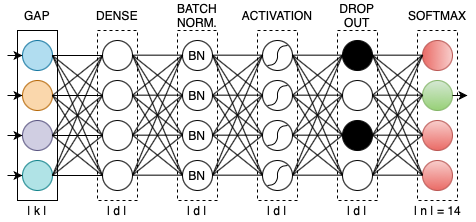
\includegraphics[width=3.3in]{img/classifier.png}
\caption{Baseline Classifier Architecture.}
\label{fig_sim}
\end{figure}

\subsubsection{Global Average Pooling Layer} this layer is introduced in order to avoid the usage of the Flatten layer, being heavier to manage in terms of complexity and parameters. While GAP is a lightweight layer able to be invariant to intrinsic shift and rotation by structural definition, gaining a more powerful generalization performance.

\subsubsection{Dense Layer} The sizes we tested for the dense layer were:
\begin{center}
\begin{tabular}{ c c }
\hline\hline
 0 (only GAP) & 98.89\% \\ 
\hline
 64 neurons & 98.79\%  \\  
 128 neurons & 98.87\%  \\
 256 neurons & \textbf{98.90\%} \\
 512 neurons & 98.79\%\\
\hline
 256 neurons (x2) & 98.89\%  \\  
\hline\hline
\end{tabular}
\end{center}

\subsubsection{Batch Normalization Layer} We introduced the batch normalization in order to have learnable parameters to be used for the regularization process.

\subsubsection{Activation Function Layer} We took into account the main three CNN activation functions in order to find the best matching one:
\begin{center}
\begin{tabular}{ c c }
\hline\hline
 ReLU & \textbf{98.87\%}  \\  
 LeakyReLU & 98.73\%  \\
 GeLU & 98.14\% \\
\hline\hline
\end{tabular}
\end{center}

\subsubsection{DropOut Layer} We tried DropOut as boosting technique; the hyperparameters we tested were:
\begin{center}
\begin{tabular}{ c c }
\hline\hline
 No DropOut & \textbf{98.93\%} \\ 
\hline
 DropOut(0.1) & 98.84\%  \\  
 DropOut(0.2) & 98.87\%  \\
 DropOut(0.3) & 98.86\% \\
\hline\hline
\end{tabular}
\end{center}

\section{Conclusion}
\subsection{Final Model}
The final model setting submitted is: \\
- \textbf{batch\_size} : 32 \\
- \textbf{loss} : Categorical Crossentropy \\
- \textbf{optimizer} : Adam(1e-4) \\
- \textbf{fine\_tuning\_layer} : 162 (\texttt{block6a\_expand\_conv})
\begin{center}
\begin{tabular}{ c | c c }
\hline
  \textbf{Layer (type)} & \textbf{Output Shape} & \textbf{Param #} \\ 
\hline\hline
 \texttt{input} & [(None, 256, 256, 3)] & 0  \\
 \texttt{efficientnetb0} & (None, 8, 8, 1280) & 4049571  \\  
 \texttt{global\_avg\_pool} & (None, 1280) & 0 \\
 \texttt{dense} & (None, 256) & 327936 \\
 \texttt{batch\_norm} & (None, 256) & 1024 \\
 \texttt{re\_lu}  & (None, 256) & 0 \\
 \texttt{softmax} & (None, 14) & 3598 \\
\hline\hline
\end{tabular}
\end{center}
\begin{center}
\begin{tabular}{ c c }
\textbf{Total params}: & 4,382,129 \\
\textbf{Trainable params}: & 3,487,786 \\
\textbf{Non-trainable params}: & 894,343 \\
\hline
\end{tabular}
\end{center}

\begin{figure}[h!]
\centering
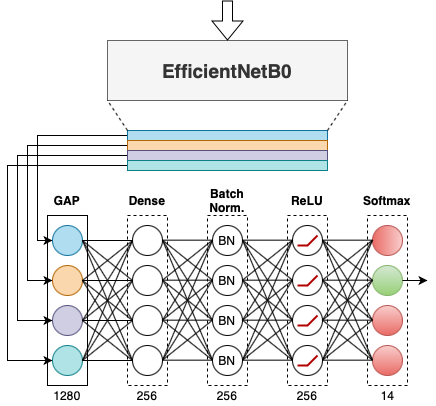
\includegraphics[width=3.3in]{img/final.png}
\caption{Final model architecture.}
\label{fig_sim}
\end{figure}

\subsection{Performance}
The dataset has been split in 80\% for training and 20\% for validation. The model in training, evaluated with an Early Stopping with patience 10 epochs based on validation loss, reached the peak of performance at epoch 34 with the following indexes:

\begin{center}
\begin{tabular}{ c c | c c }
\hline\hline
  \textbf{Train. loss} & \textbf{Train. acc.} & \textbf{Val. loss} & \textbf{Val. acc.}   \\ 
\hline
 0.0036 & 99.89\% & 0.0019 & 99.97\%  \\  
\hline\hline
\end{tabular}
\end{center}

\subsection{Confusion Matrix}
Finally, we generated the confusion matrix to identify the correctness of classification for each class with F1-score, precision and recall, on the dataset split in 60\% for training and 20\% each for validation and testing. Testing set performance indexes:

\begin{itemize}
\item \textbf{Accuracy} : 99.77\%
\item \textbf{Precision} : 99.78\%
\item \textbf{Recall} : 99.75\%
\item \textbf{F1-score} : 99.76\%
\end{itemize}

\begin{figure}[h!]
\centering
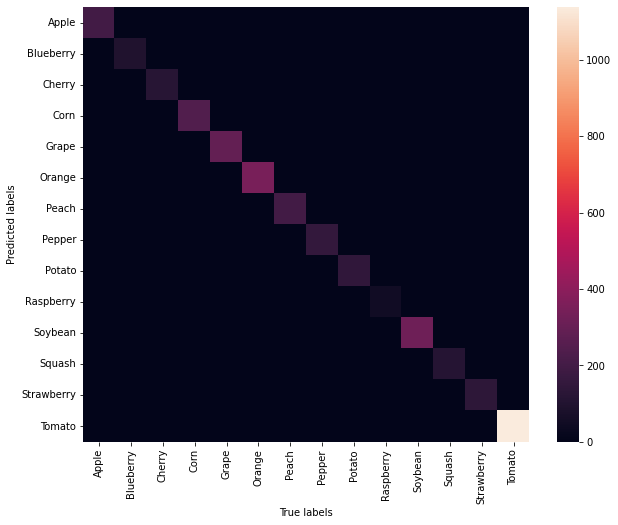
\includegraphics[width=3.5in]{img/confusion_matrix.png}
\caption{Confusion Matrix on the Testing set.}
\label{fig_sim}
\end{figure}

\subsection{Leadboard Evaluation}
\begin{itemize}
\item Development phase accuracy : \textbf{94.91\%}
\item Final phase accuracy: \textbf{94.53\%}
\end{itemize}

%\begin{thebibliography}{1}
%\bibitem{IEEEhowto:perez}
%L. Perez and J. Wang}, \emph{The Effectiveness %of Data Augmentation in Image Classification %using Deep Learning} - \relax Stanford %University, 2017.
%\end{thebibliography}

\end{document}